\chapter{Results}
\label{ch:results}


\section{Adaptive Importance Sampling Toy Model}

\section{Binary population Blck hole - Neutron star mergers}

\section{Exploring Adaptive importance Sampling}

%\section{Neutron Stars}
%Using \chromos, power colours can be obtained for a large number of observations. Applying \chromos to the population of neutron stars given in Tab.~\ref{tab:objects} reveals that most objects follow similar tracks in the \ac{PCC}~diagram. This can be seen in Fig.~\ref{fig:pc_all_ns}, where a distinct elliptical shape emerges after overplotting these tracks. In this plot $PC1$ is defined as the variance in (0.25-2.0~Hz)/(0.0039-0.031~Hz) and $PC2$ as the variance in (0.031-0.25~Hz)/(2.0-16.0~Hz). Only objects with more than three data points were included, and two objects were excluded due to their peculiar behaviours. A full discussion on the nature of those objects can be found in section~\ref{sec:dis_ns}. For sake of clarity, only points where the variance is $>\!3 \sigma$ in all four frequency bands are plotted, and error bars are omitted. Typical error bars are on the order of 17\% of the power colour values. Individual tracks can be seen more clearly in appendix~\ref{ch:pccds}, where each object has been plotted with the neutron star \ac{PCC} tracks in reference. \\
%
%While using power colours is useful in comparing evolutionary tracks of systems, power colours require two dimensions ($PC1$ and $PC2$) to classify the state of a system. Reducing this down to a single parameter can be helpful in comparing the state of a system against other parameters. To this end, the `hue'~parameter \marginpar{In colour theory, hue is defined as the attribute by virtue of which a colour is red, green, etc \citep{oed}, and is often determined using a colour wheel. This makes hue an excellent analogy to the angle within a \ac{PCC}~diagram.} can be introduced \citep{heil2015power}. Defined as the angle of a point in the \ac{PCC}~diagram with respect to a central point, hue runs in a clockwise direction from a line in the Northwest direction from $0^\circ$ to $360^\circ$. Following the original classification of the hue centre given in \citet{heil2015power}, a central point with the coordinates (4.51920, 0.453724) is chosen as reference point. An example of this classification can be seen in Fig.~\ref{fig:pc_hue_bins}, where the neutron star \ac{PCC}~diagram has been divided into hue bins of $20^\circ$. \\
%
%These hue bins allow an overview of power spectra to be created per hue bin, showing typical power spectra for a variety of objects. Comprising of various types of neutron star systems, these power spectra can be found in appendix~\ref{ch:psds}. Intrinsic scatter in the power, especially at the high frequencies, is reduced by binning data points linear in log-frequency and errors reduced accordingly. \\
%
%\begin{landscape}
%\begin{figure}
%	\myfloatalign
%	{\vspace*{-3cm}\includegraphics[width=0.8\linewidth]{pc/all_ns}}
%	\caption[Neutron stars in a \acs{PCC}~diagram]{A \ac{PCC}~diagram showing tracks for neutron stars. While providing an excellent overview of the general trend, tracks of individual objects can perhaps be best pursued in appendix~\ref{ch:pccds}, where \ac{PCC}~diagrams can be found for each system.}\label{fig:pc_all_ns}
%\end{figure}
%\end{landscape}
%
%\begin{figure}[p]
%	\myfloatalign
%	{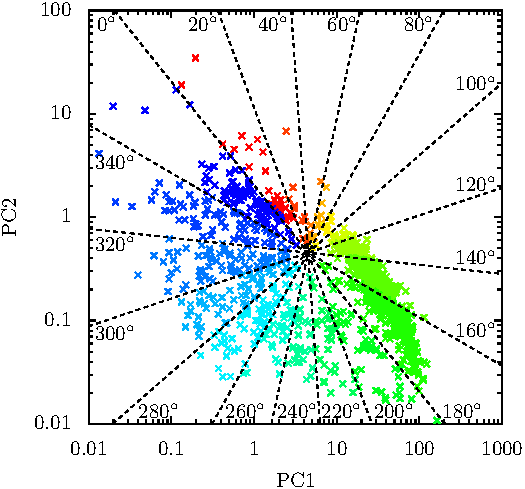
\includegraphics[width=0.8\linewidth]{pc/hue_bins}}
%	\caption[Defining the hue in a \acs{PCC}~diagram]{A \ac{PCC}~diagram showing the division of $20^\circ$ hue bins for neutron star \acp{PCC}. The starting angle is defined as the angle at $45^\circ$ in a counter-clockwise direction from the axes. Based on Fig.~2b from \citet{heil2015power}.}\label{fig:pc_hue_bins}
%\end{figure}
%
%An interesting parameter to compare hue with, is the energy spectral hardness. Linking timing information back to spectral information can provide valuable insights into properties of systems such as the relative spectral evolution and therefore changes in inner region structure. A \ac{HH}~diagram for neutron stars can be seen in Fig.~\ref{fig:hh_all_ns}, with the hardness defined as the ratio of the total count rate in 9.7-16.0~keV over the total count rate in 6.4-9.7~keV. Next to the selection methods for \ac{PCC}~points described in the first paragraph of this section, only points with a hue-error $<\!30^\circ$ are included in this graph, where errors are propagated through from the \ac{PCC}-errors. In a similar fashion to the \ac{PCC}~diagrams in appendix~\ref{ch:pccds}, individual \ac{HH}~diagrams can be found in appendix~\ref{ch:hhds}, allowing the evolution of an object within a \ac{HH}~diagram to be traced against other neutron stars.\\
%
%\begin{figure}[p]
%	\myfloatalign
%	{\includegraphics[width=\linewidth]{hh/all_ns}}
%	\caption[Neutron stars in a \acs{HH}~diagram]{A \ac{HH}~diagram showing the evolution of \ac{PCC}-tracks for neutron stars through use of the hue. Supplementary \ac{HH}~diagrams can be found in appendix~\ref{ch:hhds}, showing the tracks of individual objects with neutron star \ac{HH} tracks as reference.}\label{fig:hh_all_ns}
%\end{figure}
%
%An often-used method in X-ray astronomy to trace the overall secular evolution of \acp{LMXB} is the \ac{HI}~diagram (e.g. \citet{done2003observing}, \citet{klein2008identification} or \citet{fridriksson2015common}). In a \ac{HI}~diagram the energy spectral hardness is plotted against the relative intensity of an object. Appendix~\ref{ch:hids} shows \ac{HI}~diagrams for the full population of systems given in Tab.~\ref{tab:objects}, allowing a broad range of tracks to be compared. A number of objects show unusual tracks, a point discussed in more detail in section~\ref{sec:dis_ns}.\\
%
%In order to fully encapsulate the evolution of neutron star \acp{LMXB}, \ac{ECC}~diagrams are preferred over \ac{HI}~diagrams. The tracks in the \ac{ECC}~diagram are commonly divided into various states --- the \ac{EIS}, the \ac{IS} and the banana branch, with the \ac{LLB}, the \ac{LB} and the \ac{UB}. Linking the states of atoll source Aql~X-1 with the \ac{PCC}~diagram reveals an interesting link as shown in Fig.~\ref{fig:cc}. Here the softness is defined as the ratio of the total count rate in 3.5-6.0~keV over the total count rate in 2.0-3.5~keV, with the hardness retaining the same definition as earlier. For clarity, error bars on the energy colours have been left off the \ac{ECC}~diagram, typically being small in comparison to the \ac{ECC}~values. A clear distinction can be made in the \ac{PCC}~diagram between sources in the \ac{EIS}, and sources in the banana states. While the \ac{IS} does not show up in the \ac{PCC}~diagram, other objects showed this state to be located left of the lower apex, a region with relatively few \ac{PCC} due to the rapid state transitions.
%
%\begin{figure}[p]
%\myfloatalign%
%\makebox[\textwidth][r]{%
%\subfloat{\includegraphics[width=.5\largefigure,valign=t]{cc/ns_states_aquila_X1}}%
%\quad%
%\subfloat{\includegraphics[width=.51\largefigure,valign=t]{pc/ns_states_aquila_X1}}%
%}%
%\caption[Comparing energy and power colours]{\spacedlowsmallcaps{left} A \ac{ECC}~diagram for Aql~X-1, showing the commonly-adopted division into various states: the \acf{EIS}, the \acf{IS} and the banana branch, with the \acf{LLB}, the \acf{LB} and the \acf{UB} \spacedlowsmallcaps{right} A \ac{PCC}~diagram showing observations linked to the various states defined using the \ac{ECC}~diagram.}\label{fig:cc}
%\end{figure}
%
%\section{Neutron Stars \& Black Holes}
%In order to conduct a model-independent comparison of accreting black hole and neutron star variability, \ac{PCC}~diagrams can be constructed to show the evolution of both black hole and neutron star systems. In the left panel of Fig.~\ref{fig:ns_bh}, three representative transient black holes have been plotted for comparison with neutron stars, with additional information on these systems in Tab.~\ref{tab:objects}. Both types of system show similar paths, yet a clear distinction is found on the right-hand side of the diagram where the black holes systematically follow a higher path with respect to the neutron stars. In the right panel of Fig.~\ref{fig:ns_bh}, a \ac{HH}~diagram is shown for the same systems, where the hardness is classified as the same ratio of (9.7-16.0~keV)/(6.4-9.7~keV). With the hue washing out any radial differences in \acp{PCC}, in the \ac{HH}~diagram the black holes closely follow the neutron stars albeit with a broader coverage of angles. \\
%
%\begin{figure}[p]
%\myfloatalign%
%\makebox[\textwidth][r]{%
%\subfloat{\includegraphics[width=.51\largefigure,valign=t]{pc/ns_bh}}%
%\quad%
%\subfloat{\includegraphics[width=.49\largefigure,valign=t]{hh/ns_bh}}%
%}%
%\caption[Comparison of neutron stars and black holes]{\spacedlowsmallcaps{left} A \ac{PCC}~diagram showing black hole systems, with in grey the neutron star \acp{PCC} in Fig.~\ref{fig:pc_all_ns} as reference. \spacedlowsmallcaps{right} The same systems plotted in a \ac{HH}~diagram.}\label{fig:ns_bh}
%\end{figure}
%
%While black hole and neutron star \acp{LMXB} have similar broad-band spectral shapes, the frequency at which power spectral features occur can be a factor five higher for black holes than for neutron stars \citep{kleinwolt}. Thus comparing \ac{PCC}~values of black holes with neutron stars could perhaps best be done by shifting the frequency ranges for neutron star power colours up by a factor of five in the power spectrum. This causes the original frequency band boundaries to shift up to 0.0195, 0.155, 1.25, 10 and 64~Hz, where the final frequency is limited by the resolution in which light curves were extracted. Fig.~\ref{fig:shiftedpc} shows the result of shifting the frequency bands for neutron stars. In the left panel, the original \ac{PCC}~values for neutron stars can be seen in red against the black hole \ac{PCC}~values in grey. In the right panel are respectively the shifted \ac{PCC}~values, shown against the unaffected black hole \ac{PCC}~values. While the shifted \ac{PCC}~values show a greater overlap between neutron star and black hole \acp{PCC}, both tracks can still be distinguished.\\
%
%\begin{figure}[p]
%	\myfloatalign
%	{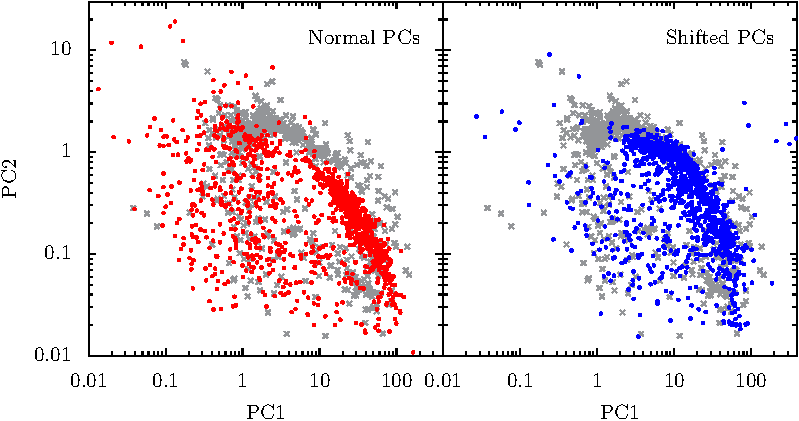
\includegraphics[width=\largefigure]{pc/shiftedpc}}
%	\caption[Effect of shifting power colour frequency bands]{\spacedlowsmallcaps{left} A \ac{PCC}~diagram showing neutron stars in red against black hole systems in grey. \spacedlowsmallcaps{right} \acp{PCC} for neutron stars where the frequency bands have been shifted up by a factor of five. The black hole systems in grey have retained the original frequency bands for their \ac{PCC} values.}\label{fig:shiftedpc}
%\end{figure}
%
%\section{Effects of Neutron Star Properties}
%
%\enlargethispage{2\baselineskip}
%\subsection{Inclination}
%Power colours present the unique ability to compare various parameters of multiple systems throughout different energy spectral states. Using power colours in such a fashion, \citet{heil2015inclination} found black holes systems followed an inclination-dependent track in the \ac{HH}~diagram. Applying the same technique to neutron stars results in Fig.~\ref{fig:inclination}, where sources have been split into either a low ($i\!\leq\!60^\circ$)  or high ($i\!>\!60^\circ$) binary orbit inclination group using Tab.~\ref{tab:objects}, following the division adopted in \citet{heil2015inclination}. Errorbars have been omitted for clarity and sources with an undefined inclination plotted in grey. While no particular trend can be discerned from the \ac{PCC}~diagram, the resulting \ac{HH}~diagram shows signs of an offset dependent on inclination, with low inclination sources showing higher hardness per hue than high inclination sources. Implications of this trend are discussed in section~\ref{sec:dis_incl}, including suggestions on possible origins.\\
%
%\begin{figure}[p]
%\myfloatalign%
%\makebox[\textwidth][l]{%
%\subfloat{\includegraphics[width=.51\largefigure,valign=t]{pc/inclination}}%
%\quad%
%\subfloat{\includegraphics[width=.49\largefigure,valign=t]{hh/inclination}}%
%}%
%\caption[Inclination effects]{\spacedlowsmallcaps{left} A \ac{PCC}~diagram with neutron star systems split into high and low inclination groups. Sources with an undefined inclination have been plotted in grey. Details on the inclination of individual sources can be found in Tab.~\ref{tab:objects}. \spacedlowsmallcaps{right} A \ac{HH}~diagram with neutron star systems divided in the same manner.}\label{fig:inclination}
%\end{figure}
%
%\subsection{Atoll \& Z Sources}
%Based on the path \acp{LMXB} trace out in a \ac{ECC}~diagram, neutron star systems can be classified into two subclasses: atoll and Z sources \citep{hasinger1989two}. In Tab.~\ref{tab:objects}, systems classified as either an atoll or a Z source have been denoted with respectively an $A$ or a $Z$. A comparison of these systems in the \ac{PCC} and \ac{HH}~space can be seen in Fig.~\ref{fig:atoll_z}. Plotted together with unclassified neutron stars, the Z sources in the \ac{PCC}~diagram rarely cross into the upper-right half of diagram. This is reflected in the \ac{HH}~diagram, where almost all Z source values remain above a hue of $180^\circ$. No particular difference can be discerned between atoll and as of yet unclassified sources, with atoll sources tracing a similar path to the latter.\\
%
%\begin{figure}[p]
%\myfloatalign%
%\makebox[\textwidth][l]{%
%\subfloat{\includegraphics[width=0.51\largefigure,valign=t]{pc/atoll_z}}%
%\quad%
%\subfloat{\includegraphics[width=0.49\largefigure,valign=t]{hh/atoll_z}}%
%}%
%\caption[Comparing Atoll and Z sources]{\spacedlowsmallcaps{left} \ac{PCC}~diagram with systems classified as atoll sources in red, Z sources in blue and unclassified sources in grey. An overview showing the type of each individual system can be found in Tab.~\ref{tab:objects}. \spacedlowsmallcaps{right} Replotting the same systems in a \ac{HH}~diagram.}\label{fig:atoll_z} % \TODO Check Z-source outlier
%\end{figure}
%
%A further division can be made in Z sources on the basis of spectral and timing behaviour, allowing sources to be split into Cyg- and Sco-like sources \citep{kuulkers1997gx}. Nonetheless, there are only a few sources which have been classified as Cyg- or Sco-like sources, as seen in Tab.~\ref{tab:objects}. These can be plotted in a \ac{PCC}~diagram, as seen in Fig.~\ref{fig:pc_sco_cyg}. With Z sources rarely straying beyond the lower left corner, a large degree of scatter is expected, and is found in the \ac{PCC}~values. It is interesting that there is seemingly a lower degree of scatter for the Cyg-like sources in comparison to the Sco-like sources.\\
%
%\begin{figure}[p]
%	\myfloatalign
%	{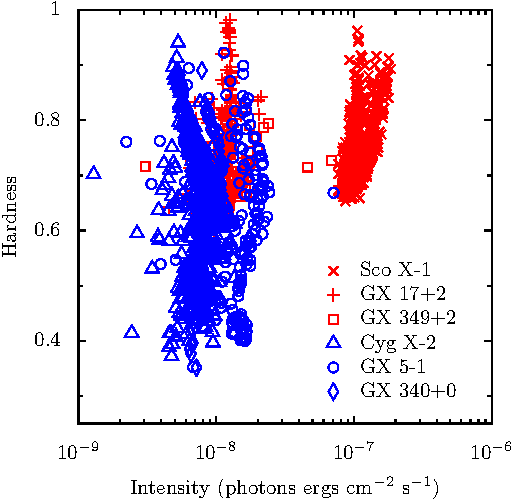
\includegraphics[width=0.8\linewidth]{pc/sco_cyg}}
%	\caption[\acs{PCC}~diagram with Sco- and Cyg-like sources]{\ac{PCC}~diagram with Z sources. Sco-like sources are plotted in red and with Cyg-like sources in blue. Note the large contributions of Sco X-1 and Cyg X-2 to each respective group.}\label{fig:pc_sco_cyg}
%\end{figure}
%
%\subsection{Pulsations \& Spin}
%Since the discovery of the first \ac{AMSP} by \citet{wijnands1998millisecond}, systematic searches have revealed fourteen other systems of this nature \citep[see][for a review]{patruno2012accreting}. One such source, HETE J1900.1-2455, was the first to show `quasi-persistent' activity \citep{galloway2006intermittent}. Believed to be due to a build-up and subsequent suppression of magnetic field through channeling of the accreting flow \citep[e.g.][]{cumming2001magnetic}, it provides an effective test for a possible correlation between magnetic fields and \acp{PCC}. Fig.~\ref{fig:hete_pulsations} shows a selection of observations split into time intervals of standard luminosity levels and time intervals with pulsations. Selections were made on basis of the fractional pulse amplitudes between MJD~53520--53690 as given in \citet{galloway2006intermittent}. Though the \ac{PCC}~diagram hints at higher PC2 values during pulsation periods, no conclusive correlation can be determined, with relatively few observations available to distinguish any trends.\\
%
%\begin{figure}[p]
%	\myfloatalign
%	{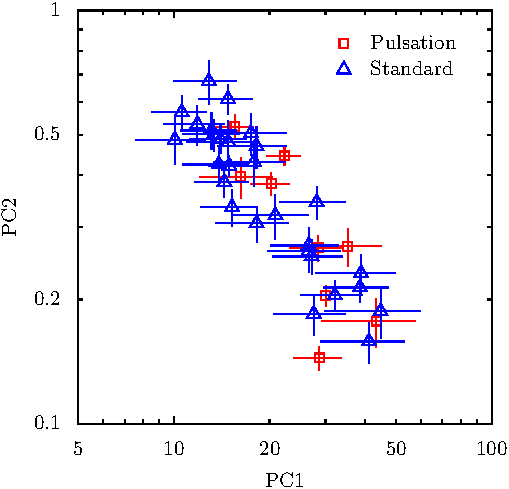
\includegraphics[width=0.8\linewidth]{pc/hete_pulsations}}
%	\caption[\acsp{PCC} during intermittent pulsations]{A \ac{PCC}~diagram with observations of HETE~J1900.1-2455 split into pulsation time intervals and periods of standard flux-levels. The division between these time intervals was made on basis of information in \citet{galloway2006intermittent}.}\label{fig:hete_pulsations}
%\end{figure}
%\newpage
%Pulsations in neutron star \acp{LMXB} are commonly used in an attempt to establish the spin frequency of the neutron star, resulting in groups of objects referred to as respectively bursters and pulsars. It is generally accepted that the rapid increase in flux observed in bursters is linked to unstable nuclear burning on the neutron-star surface \citep[e.g.][]{klis2000millisecond}, providing a means to determine the spin frequency of the neutron star through hotspots on the neutron star surface \citep[see][]{chakrabarty2003nuclear,strohmayer2003new}. In contrast, pulsars show regular pulsations, resulting in extremely precise spin frequencies. While spin frequencies typically fall far from the frequency bands that power colours probe, some effect of the higher spin frequencies could perhaps be expected to be seen in the lower power colour frequencies. The spin could for instance affect the accretion flow via the pulsar magnetosphere. Coupling spin frequencies with \acp{PCC} results in Fig.~\ref{fig:spin}, with objects colour-coded according to their spin frequency. Objects with less than four points have been removed from the sample, to ensure clarity. Bursters show no distinct effects on \acp{PCC}, however a tentative link could perhaps be found in pulsar systems where a shift in \acp{PCC} according to spin frequency can be observed. An in-depth discussion on this relation can be found in section~\ref{sec:dis_ps}, as well as an hypothesis on the origin of this tentative relationship.\\
%
%\begin{figure}[p]
%	\myfloatalign
%	\makebox[\textwidth][l]{%
%	{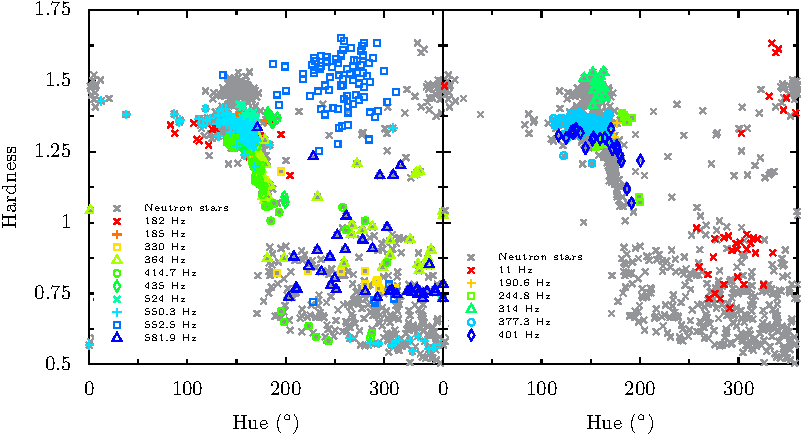
\includegraphics[width=\largefigure]{pc/bursters_pulsars}}
%	}%	
%	\caption[The effect of spin frequency on \acsp{PCC}]{\spacedlowsmallcaps{left} Bursters plotted in order of frequency, with neutron star \acp{LMXB} without a defined spin frequency in comparison. \spacedlowsmallcaps{right} \ac{PCC}~diagram showing pulsars per spin frequency together with the \ac{PCC} values of the other neutron stars.}\label{fig:spin}
%\end{figure}